\documentclass[a4paper,dvipsnames]{article}

\input ../header
\newcommand{\checkedbox}{\makebox[0pt][l]{$\square$}\raisebox{.15ex}{\hspace{0.1em}$\checkmark$}}
\newcommand{\checkbox}{\makebox[0pt][l]{$\square$}\raisebox{.15ex}{\hspace{0.1em}}\hspace{3mm}}

\usepackage{gensymb}

\begin{document}

\title{Activité -- Distance entre deux nombres et valeur absolue}

\date{}
\author{}

\maketitle{}

\thispagestyle{empty}
\pagestyle{empty}

\section{Distance entre deux nombres}

\begin{enumerate}
  \item 
    \begin{enumerate}
      \item Déterminer le nombre d'années pendant lesquelles chacun des hommes suivants a vécu : Aristote (384-322 av. J.-C.), Victor Hugo (1802-1885).\rep{3}
      \item Le désert de Qumran, près de la mer Morte, a été occupé par les Esséniens de 152 avant J.-C. à 68 après J.-C. Combien d'années a duré l'occupation ?\rep{3}
      \item Pythagore a vécu 80 ans et il est mort en 480 avant J.-C. En quelle année est-il né ?\rep{3}
    \end{enumerate}
  \item Dans un jeu vidéo, un personnage se déplace le long d'un chemin rectiligne. On a représenté sur la droite numérique ci-dessous quelques éléments de l'écran.
    \begin{center}
      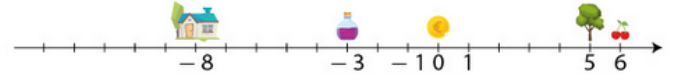
\includegraphics[width=12cm]{1_4_activite_introduction_jeu_video.png}
    \end{center}
    \begin{enumerate}
      \item 
	\begin{enumerate}
	  \item Quelle est la distance entre les cerises et la pièce d'or ? On dit qu'il s'agit de la distance entre $6$ et $0$.\rep{2}
	  \item Quelle est la distance entre $-8$ et $0$ ?\rep{2}
	\end{enumerate}
      \item On note $x$ l'abscisse de la position du personnage sur cette droite.
	\begin{enumerate}
	  \item Exprimer en fonction de $x$ la distance entre $x$ et $0$ selon la position du personnage par rapport à la pièce d'or.\rep{2}
	  \item Que représente la distance entre $x$ et $5$ ?\rep{2}
	  \item Exprimer cette distance en fonction de $x$ en envisageant deux cas.\rep{3}
	\end{enumerate}
      \item À un moment donné, le personnage est à égale distance de $-3$ et de $5$. Quelle est la valeur de $x$ dans ce cas ?\rep{2}
      \item Le personnage est invincible lorsque sa distance à $-8$ est inférieure ou égale à $3$.
	\begin{enumerate}
	  \item Colorier cette zone d'invincibilité en rouge.
	  \item Décrire cette zone d'invincibilité à l'aide de $x$ et d'un intervalle.\rep{2}
	\end{enumerate}
    \end{enumerate}
  \item 
    \begin{enumerate}
      \item Placer sur une droite numérique d'origine $O$ les points $A$ d'abscisse $5$ et $B$ d'abscisse $-4$.\rep{3}
	% Placer sur une droite numérique d'origine $O$ les points $A$ d'abscisse $5$, $B$ d'abscisse $2$, $C$ d'abscisse $-3$ et $D$ d'abscisse $-2$.\rep{4}
%      \item Lire sur le graphique les distances $BA$, $BC$ et $CD$.\rep{3}
%      \item Quelle opération faut-il faire pour calculer les distances $OC$, $CA$ et $BC$ ?\rep{3}
%      \item Soient $E$ et $F$ deux points de la droite d'abscisses respectives $0,85$ et $\dfrac{14}{3}$. Calculer les distances $BE$ et $BF$.\rep{3}
      \item 
	\begin{enumerate}
	  \item Représenter en vert l'ensemble des points qui se trouvent à une distance de $A$ strictement inférieure à $2,5$.
	  \item À quel ensemble appartiennent les abscisses de ce points ?\rep{2}
	\end{enumerate}
      \item 
	\begin{enumerate}
	  \item Représenter en rouge l'ensemble des points qui se trouvent à une distance de $B$ supérieure ou égale à $3$.
	  \item À quel ensemble appartiennent les abscisses de ces points ?\rep{2}
	\end{enumerate}
    \end{enumerate}
\end{enumerate}

\section{Racine carrée et carré}

On considère les deux programmes de calcul ci-dessous:

\begin{multicols}{2}
  \begin{enumerate}
    \item[] \textbf{Programme de calcul 1}
      \begin{algorithmic}[1]
	\State Élever au carré
	\State Prendre la racine carrée
      \end{algorithmic}
    \item[] \textbf{Programme de calcul 2}
      \begin{algorithmic}[1]
	\State Prendre la racine carrée
	\State Élever au carré
      \end{algorithmic}
  \end{enumerate}
\end{multicols}

\begin{enumerate}
  \item Peut-on appliquer ces programmes de calcul aux nombres $9$, $7$, $-16$, $0$ ?\rep{4}
  \item 
    \begin{enumerate}
      \item À quels réels peut-on appliquer chacun de ces programmes de calcul ?\rep{2}
      \item Écrire en fonction de $x$ le résultat obtenu pour chacun de ces programmes.\rep{4}
    \end{enumerate}
  \item Donner un algorithme qui permet de calculer le résultat du programme de calcul $1$ sans utiliser la racine carrée.\rep{3}
\end{enumerate}

\end{document}
